\documentclass[tikz,border=10pt]{standalone}
\usetikzlibrary{calc, intersections}

\begin{document}
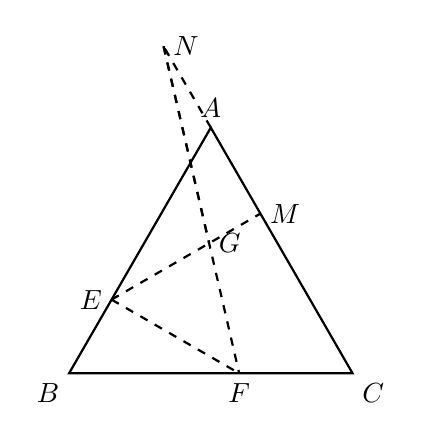
\begin{tikzpicture}[scale=1.2, >=stealth]
    % 1. 定义主要顶点
    % 基于图像比例：设底边 BC 水平，A 在上方
    \coordinate (B) at (0,0);
    \coordinate (C) at (3,0);
    \coordinate (A) at (1.5,2.6);

    % 2. 定义边上的点
    % E 在 AB 上，M 在 AC 上，F 在 BC 上
    \coordinate (E) at ($(B)!0.3!(A)$);
    \coordinate (M) at ($(A)!0.35!(C)$);
    \coordinate (F) at ($(B)!0.6!(C)$);
    \coordinate (N) at (1,3.46);

    % 3. 定义辅助线交点
    % G 是 EM 与 AF 的交点
    \coordinate (G) at (intersection of E--M and F--N);
    

    

    % 5. 绘制实线（三角形主体）
    \draw[thick] (A) -- (B) -- (C) -- cycle;

    % 6. 绘制虚线（辅助线）
    \draw[dashed, thick] (E) -- (M);    % 线段 EM
    \draw[dashed, thick] (E) -- (F);    % 线段 EF
    \draw[dashed, thick] (N) -- (F);    % 线段 AF (含 G 点)
    \draw[dashed, thick] (A) -- (N);    % A 到 N 的延长部分
    \draw[dashed, thick] (N) -- (G);    % N 到 G 的特殊连线（根据图示虚线轨迹）

    % 7. 标注顶点标签
    % 使用 [position] 微调标签位置，确保不被线条遮挡
    \node[above] at (A) {$A$};
    \node[below left] at (B) {$B$};
    \node[below right] at (C) {$C$};
    \node[left] at (E) {$E$};
    \node[right] at (M) {$M$};
    \node[below] at (F) {$F$};
    \node[right] at (G) {$G$};
    \node[right] at (N) {$N$};



\end{tikzpicture}
\end{document}